\newpage
\section{Подсистема журналирования}

Система журналирования – это внешний модуль, позволяющий вести лог следующих событий в ФТМИС:
\begin{itemize}
 \item Авторизация пользователя в системе;
 \item Печать документа;
 \item Cоздание, удаление, изменение типов действий;
 \item Создание, удаление, изменение событий;
 \item Создание, удаление, изменение действий;
 \item Ошибки, связанные с ошибками работы, обращениями в БД.
\end{itemize}

\begin{figure}[ht]\centering
 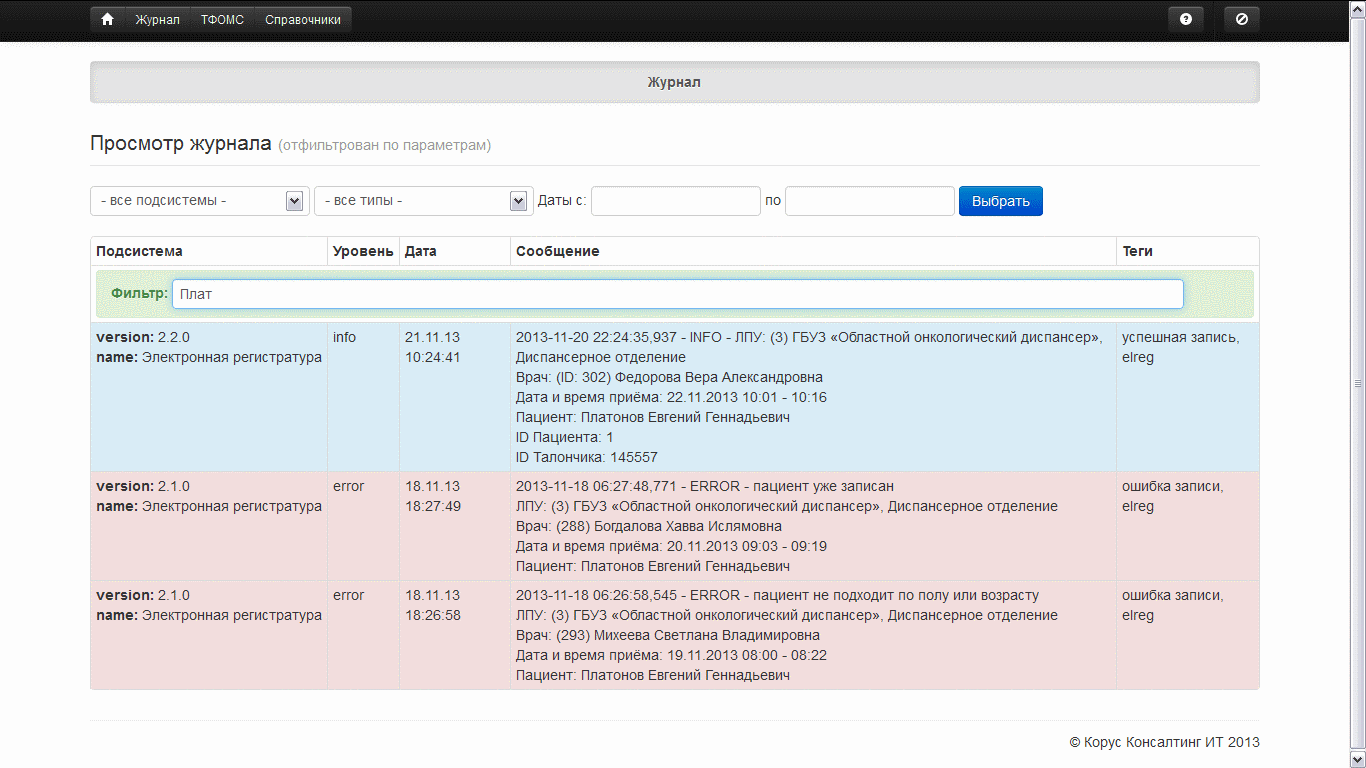
\includegraphics[width = 1\textwidth ,keepaspectratio]{log_jur}
 \caption{Журнал событий}
 \label{img_log_jur}
\end{figure} 
 
Для ведения лога необходимо, чтобы журналирование событий было включено на стороне ФТМИС.

Система администрирования ЛПУ позволяет просматривать описанный выше лог в удобном виде, дает возможность фильтровать события по различным параметрам.

Для перехода к просмотру журнала событий необходимо нажать кнопку \btn{Журнал} на панели управления. Будет осуществлен переход на страницу просмотра журнала (Рисунок \ref{img_log_jur}).

По умолчанию отображаются последние 100 записей лога событий. Данные представлены в виде таблицы, имеющей следующие столбцы:
\begin{itemize}
 \item В столбце \dm{Подсистема} представлена информация о рабочей станции и пользователе, инициировавшем событие. Указывается IP-адрес рабочей станции (\dm{IP}), название рабочей станции/имя компьютера (\dm{host}), версия клиентской части ФТМИС, с помощью которой было совершено данное событие (\dm{version}) и имя пользователя, под которым был осуществлен вход в ФТМИС (\dm{user}).
 \item В столбце \dm{Уровень} указывается уровень значимости сообщения. Выделяются следующие уровни (от наиболее важного к наименее значимому):
 \begin{itemize}
  \item Critical – критические ошибки, возникающая в процессе работы или при обращении к базе данных.
  \item Error – ошибка, возникающая в процессе работы или при обращении к базе данных. Записи данного типа окрашены в розовый цвет.
  \item Warning – предупреждения, возникающая в процессе работы или при обращении к базе данных.
  \item Notice – записи лога об успешно совершенных событиях. К данной группе относятся записи о совершении входа в систему, печати документов, создании, изменении, удалении типов действий и событий. Записи данного типа окрашены в голубой цвет.
  \item Note – аналогично предыдущему, запись лога о совершенных стандартных событиях. В данной группе относятся данные о записи пациентов на прием, создании, изменении, удалении действий. Записи данного типа окрашены в голубой цвет.
  \item Debug – сообщения, используемые для отладки работы системы (разработчиками). Записи данного типа окрашены в белый цвет.
 \end{itemize}
 \item В столбце \dm{Дата} указывается дата и время совершения указанного события. Время может браться с сервера системы журналирования либо из ФТМИС в зависимости от настроек.
 \item В столбце \dm{Сообщение} отображается краткая информация о совершенном событии. Как правило, в поле содержится название события, идентификатор и фамилия пациента, медицинские записи которого подвергались обработке. Состав информации в данном поле определяется типом информационного сообщения. Например, сообщение о входе пользователя в систему содержит только название, а сообщение о записи пациента на прием содержит код и название ЛПУ и фамилию врача, к которому записывается пациент; дату и время, на которые осуществлена запись; идентификатор и фамилию пациента, а так же идентификатор выданного талона. Для событий уровня critical или error в данном поле может содержаться текст ошибки.
 \item В столбце \dm{Теги} указываются основные ключевые слова для данного события. Теги привязаны к виду события. Соответственно, события одного вида имеют одни и те же теги.
\end{itemize}
 
Для отбора записей лога по определенным параметрам можно воспользоваться фильтром. Фильтр предусмотрен по полям: \dm{Подсистема}, \dm{Уровень}, \dm{Дата}.

В поле \dm{Подсистема} можно выбрать определенное сочетание (рабочая станция – имя пользователя). Тогда после применения фильтра будут отображаться только события совершенные выбранным пользователем с выбранной рабочей станции.

В следующем поле можно выбрать уровень события (critical, error, warning, notice, note, debug). Если в поле ничего не выбрано, то в таблице отображаются события всех уровней.

В полях \dm{Дата с} \dm{по} указываются даты начала и окончания периода, за который необходимо отобразить лог событий. Дату можно выбрать из календаря или ввести с клавиатуры. Календарь раскрывается при установке курсора в поле для ввода даты.

После того как параметры фильтра установлены, необходимо нажать кнопку \btn{Выбрать} справа от полей задания параметров фильтрации. Данные лога событий будут отфильтрованы в соответствии с указанными параметрами.

Ниже находится еще одна строка, с помощью которой можно фильтровать данные – поле \dm{Фильтр}. Но если фильтр, описанный ранее (далее основной фильтр), позволяет выбрать любые данные из лога согласно параметрам фильтрации, то строка \dm{Фильтр} (или строка фильтрации) позволяет выбирать данные только среди записей, отображенных на экране на момент ввода данных в строку фильтрации. Фильтрация записей в таблице происходит автоматически по мере ввода данных в строку \dm{Фильтр}. В результат фильтрации попадут записи, в любой из ячеек которых встречается буквосочетание, введенное в строку фильтрации. Для снятия данного фильтра достаточно очистить поле \dm{Фильтр}. Тогда на экране снова будут отображаться записи, выбранные с помощью основного фильтра.
